\section{A polynomial with a weakly expanding conjugate pair}
\label{np:section}

The final example uses a polynomial with one conjugate pair just outside the
unit circle. We will prove singularity directly by counting typical prefixes.
Counting all polynomial values in their conjugate coordinates
therefore gives slightly too many possible prefixes. We obtain the required
improvement by a product of positive trigonometric factors: its integral in the expanding
coordinates stays bounded, whereas it grows exponentially on a set of words
whose probability tends to one.

Throughout this section, every terminating decimal denotes the corresponding
exact rational number. Put
\begin{equation}
 p(t)=t^{31}-2t^{30}+\sum_{j=0}^{9}(t^{3j+1}-t^{3j}).
 \label{np:polynomial}
\end{equation}
The identity
\begin{equation}
 (t^2+t+1)p(t)=t^{33}-t^{32}-t^{31}-t^{30}-1
 \label{np:relation}
\end{equation}
will control the near-cancellations in the trigonometric product.

\begin{theorem}\label{np:main}
The polynomial \(p\) in \eqref{np:polynomial} has a unique real root
\(\beta\in(1.8392,1.8393)\). This root is not a Pisot number, and
\(\nu_{1/\beta}\) is singular with respect to Lebesgue measure.
\end{theorem}

We first record the root bounds needed in the proof. The proposition is
proved by rational root disks in Section~\ref{cert:roots}.

\begin{proposition}[Root bounds]\label{np:roots}\label{np:root-data}
All roots of \(p\) are simple. Its roots outside the unit circle are
\(\beta,\alpha,\overline\alpha\), where \(\beta\) is real,
\(\operatorname{Im}\alpha>0\), and
\begin{equation}
 \begin{gathered}
  1.8392<\beta<1.8393,\qquad
  1.0002089<|\alpha|^2<1.0002094,\\
  |\alpha|^{-1}<0.9999.
 \end{gathered}
 \label{np:root-bounds}
\end{equation}
The remaining roots are fourteen nonreal conjugate pairs, each of modulus
less than \(0.994\).
\end{proposition}

Write \(D=\{\beta,\alpha,\overline\alpha\}\) and let \(I\) be the set of
remaining roots. The expanding volume factor is
\begin{equation}
 \mathcal M=\prod_{r\in D}|r|=\beta|\alpha|^2,
 \qquad \log\mathcal M<\log\beta+0.0002094.
 \label{np:mahler}
\end{equation}
The last inequality uses \(\log(1+u)<u\) for \(u>0\).

The root bounds already show that \(\beta\) is not Pisot. Indeed, suppose
\(\beta\) were Pisot, and divide \(p\) by its monic minimal polynomial.
The quotient is monic and integral, has constant term of absolute value one,
and contains \(\alpha,\overline\alpha\) among its roots but not \(\beta\).
The product of the moduli of its roots is greater than one if it has no roots
in \(I\), and otherwise is at most
\(1.0002094\cdot0.994<1\). Both conclusions contradict the constant term.
It remains to prove singularity.

\subsection{Word vectors and characters}
\label{np:characters-section}

For a word \(a=(a_0,\ldots,a_{N-1})\in\{0,1\}^N\), define
\begin{equation}
 y_r(a)=\sum_{j=0}^{N-1}a_jr^j\quad(r\in D\cup I),
 \qquad x_r(a)=r^{-N}y_r(a)\quad(r\in D).
 \label{np:word-coordinates}
\end{equation}
Vectors indexed by roots are always constrained by
\(y_{\overline r}=\overline{y_r}\), and a conjugate pair counts as one complex
coordinate, or two real coordinates. In particular, the space of all
\(y\)-vectors has real dimension \(31\).

\begin{lemma}\label{np:lattice}
All vectors \(y(a)\), for all \(N\) and all words \(a\), belong to a fixed
full lattice in this real vector space. Their contracting coordinates
\((y_r)_{r\in I}\) and normalized expanding coordinates \((x_r)_{r\in D}\)
lie in fixed bounded boxes. The change from \((x_D,y_I)\) to \((y_D,y_I)\)
has real Jacobian determinant of absolute value \(\mathcal M^N\).
\end{lemma}

\begin{proof}
Reduction of \(\sum a_jt^j\) modulo the monic polynomial \(p\) gives an
integer coefficient vector of length \(31\). Evaluation at the roots is an
invertible real-linear map: a polynomial of degree at most \(30\) that
vanishes at all \(31\) distinct roots is zero. The image of \(\Z^{31}\)
under this map is the required lattice. No irreducibility assumption is
needed. The bounds follow from
\[
 |y_r(a)|\le\frac1{1-|r|}\quad(r\in I),\qquad
 |x_r(a)|\le\frac1{|r|-1}\quad(r\in D).
\]
Multiplication of the real coordinate by \(\beta^N\) and of the complex
coordinate by \(\alpha^N\) has determinant
\(\beta^N|\alpha|^{2N}=\mathcal M^N\).
\end{proof}

To distinguish the word vectors from typical points of these boxes, define
the real sequences
\begin{equation}
 C_0(m)=
 \begin{cases}
  \displaystyle\sum_{r\in I}\frac{r^{-1-m}}{p'(r)},&m<0,\\[4pt]
  \displaystyle-\sum_{r\in D}\frac{r^{-1-m}}{p'(r)},&m\ge0,
 \end{cases}
 \qquad C_1(m)=C_0(m+3)-C_0(m)+C_0(m-1).
 \label{np:coefficients}
\end{equation}
Partial fractions give
\[
 \frac1{p(t)}=\sum_{m\in\Z}C_0(m)t^m,
 \qquad \max_{r\in I}|r|<|t|<\min_{r\in D}|r|.
\]
Thus \(C_0\) is the bilateral Laurent coefficient sequence of \(1/p\), and
both \(C_0,C_1\) decay exponentially at both ends. The same inversion by an
exponentially decaying two-sided sequence is used by Lind and Schmidt
\cite[Lemma~4.5 and Example~4.7]{LindSchmidt1999} to construct homoclinic points for algebraic
actions. Here the explicit root formula will give characters adapted to the
word vectors.

For arbitrary expanding
coordinates \(x_D\), with \(x_\beta\in\R\) and
\(x_{\overline\alpha}=\overline{x_\alpha}\), put
\begin{equation}
 \begin{split}
 Z_i^{(0,N)}(x)
 &=\exp\!\left(-2\pi\mathrm i\sum_{r\in D}
                   \frac{x_rr^i}{p'(r)}\right)
   \exp\!\left(-\pi\mathrm i\sum_{k=0}^{N-1}C_0(k-i)\right),\\
 Z_i^{(1,N)}(x)
 &=Z_{i-3}^{(0,N)}(x)\overline{Z_i^{(0,N)}(x)}Z_{i+1}^{(0,N)}(x),
 \qquad i\in\Z.
 \end{split}
 \label{np:characters}
\end{equation}
These functions have modulus one.

\begin{lemma}[Characters at word vectors]\label{np:word-character}
If \(b_k=a_{N-1-k}\), then for \(A\in\{0,1\}\) and \(i\in\Z\),
\begin{equation}
 Z_i^{(A,N)}(x(a))
 =\exp\!\left(\pi\mathrm i\sum_{k=0}^{N-1}
                     C_A(k-i)(2b_k-1)\right).
 \label{np:word-character-formula}
\end{equation}
\end{lemma}

\begin{proof}
The reversed word gives \(x_r(a)=\sum_{k=0}^{N-1}b_kr^{-1-k}\).
For each integer \(l\ge0\), Lagrange interpolation shows that
\[
 \sum_{r\in D\cup I}\frac{r^l}{p'(r)}
\]
is the coefficient of \(t^{30}\) in the remainder of \(t^l\) modulo \(p\),
and hence is an integer. Consequently, when \(m<0\), the coefficient
\(-\sum_{r\in D}r^{-1-m}/p'(r)\) differs from \(C_0(m)\) by an integer.
Its contribution to the exponent with coefficient \(2\pi\mathrm i b_k\)
is unchanged by this replacement. When \(m\ge0\), the coefficients
already agree. The second factor in \eqref{np:characters} supplies the
centering by \(-1\), proving the formula for \(A=0\). Multiplication of
the three characters proves it for \(A=1\).
\end{proof}

The corresponding stationary model uses independent fair bits
\((b_k)_{k\in\Z}\) and the unit random variables
\begin{equation}
 \mathcal Z_i^{(A)}=
 \exp\!\left(\pi\mathrm i\sum_{k\in\Z}C_A(k-i)(2b_k-1)\right).
 \label{np:stationary}
\end{equation}
The series converges absolutely. Independence gives the real moments
\begin{equation}
 \begin{split}
 P_A&=\E\mathcal Z_i^{(A)}
       =\prod_{m\in\Z}\cos(\pi C_A(m)),\\
 P_{AB}^{\pm}(k)
   &=\E\bigl[\mathcal Z_i^{(A)}
                    (\mathcal Z_{i-k}^{(B)})^{\pm1}\bigr]\\
   &=\prod_{m\in\Z}\cos\bigl(\pi(C_A(m)\pm C_B(m+k))\bigr),
 \qquad k\ge0.
 \end{split}
 \label{np:scalar-products}
\end{equation}

\subsection{A predictor with a positive mean gain}
\label{np:predictor-section}

The weakly expanding pair produces long decaying tails in \(C_0\).
Some shifted tails nearly cancel in the signed products
\(P_{00}^{\pm}(k)\). A linear combination of the corresponding phases will
use these correlations. For rational weights \(w_{ks}\), define
\begin{equation}
 \begin{split}
 G_i^{(N)}(x)
  &=-0.001+0.0055 Z_{i-33}^{(1,N)}(x)
    +\sum_{k=30}^{2000}\sum_{s=0}^1
           w_{ks}\bigl(Z_{i-k}^{(0,N)}(x)\bigr)^{1-2s},\\
 \mathcal G_i
  &=-0.001+0.0055\mathcal Z_{i-33}^{(1)}
    +\sum_{k=30}^{2000}\sum_{s=0}^1
           w_{ks}(\mathcal Z_{i-k}^{(0)})^{1-2s},\\
 \mathcal L_i&=\operatorname{Re}(\mathcal Z_i^{(0)}\mathcal G_i).
 \end{split}
 \label{np:predictor}
\end{equation}

\begin{proposition}[Predictor estimates]\label{np:moments}\label{np:moment-bounds}
There exist weights \(w_{ks}\in10^{-9}\Z\), indexed by
\(30\le k\le2000\) and \(s\in\{0,1\}\), such that
\begin{equation}
 0.001+0.0055+\sum_{k,s}|w_{ks}|
   =\frac{198442946}{10^9}<x_*:=0.199
 \label{np:weight-sum}
\end{equation}
and, in the stationary model,
\begin{equation}
 \begin{gathered}
 \E\mathcal L_i>0.000210,\qquad
 \E|\mathcal G_i|^2<0.000145,\\
 \left|\E\bigl[(\mathcal Z_i^{(0)})^2\mathcal G_i^2\bigr]\right|
     <0.000007.
 \end{gathered}
 \label{np:moment-estimates}
\end{equation}
In particular, \(|G_i^{(N)}(x)|\le x_*\) for every \(N,i,x\), and
\(|\mathcal G_i|\le x_*\) for every bit sequence.
\end{proposition}

We fix weights supplied by Proposition~\ref{np:moments}. Their exact
rational construction is given in Section~\ref{cert:algorithm}, and the
moment bounds are proved in Section~\ref{cert:moments}.

The next two subsections construct a positive product whose logarithm has a
positive mean under this stationary model and whose integral is bounded in
the expanding coordinates. These two estimates will remove
an exponential proportion of the lattice points allowed by
Lemma~\ref{np:lattice}.

\subsection{Damping the possible frequency cancellations}
\label{np:damping-section}

Choose a fixed integer \(i_0\ge1\) so that
\begin{equation}
 \frac{0.1\beta^{i_0}}{|p'(\beta)|}>1.
 \label{np:initial-index}
\end{equation}
For a word length \(N\), use every complete block
\[
 B_q=\{i_0+22q,\ldots,i_0+22q+20\}\subseteq\{0,\ldots,N-1\},
 \qquad q\ge0,
\]
and write \(J_N\) for their union. Thus each block has \(21\) indices and
consecutive blocks are separated by one unused index.

The near-relation \eqref{np:relation} dictates which signed digit patterns
need to be retained when integrating a block. For a pattern
\((d_i)_{i\in B_q}\in\{-1,0,1\}^{B_q}\), let \(b=\max B_q\) and set
\[
 v_i=\beta^{-i}\sum_{j=i}^{b}d_j\beta^j,\qquad
 v_{b+1}=0.
\]
Reading from the largest index downwards gives
\(v_i=\beta v_{i+1}+d_i\). At the root \(\beta\),
\eqref{np:relation} becomes
\begin{equation}
 \beta^3-\beta^2-\beta-1=\beta^{-30}.
 \label{np:near-cubic}
\end{equation}
In particular, the four digits
\([\sigma,-\sigma,-\sigma,-\sigma]\) leave the small normalized remainder
\(\sigma\beta^{-30}\). We encode these approximate returns by the
transitions in Figure~\ref{np:automaton}. The initial
state is \(0\), and the permitted terminal states are \(0,C_+,C_-\).
For each sign \(\sigma\in\{-1,1\}\), the numerical values assigned to the
states are
\begin{equation}
 0,\qquad A_\sigma:\ \sigma,\qquad
 B_\sigma:\ \sigma(\beta-1),\qquad
 C_\sigma:\ \sigma(\beta^2-\beta-1).
 \label{np:state-values}
\end{equation}
A pattern is called \emph{admissible} if every transition is allowed and
its terminal state is permitted.

\begin{figure}[ht]
 \centering
 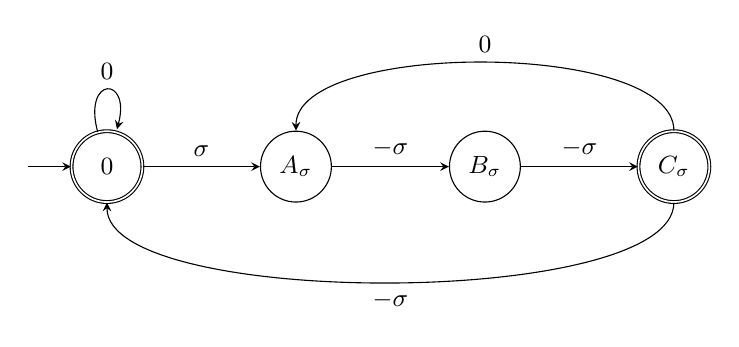
\begin{tikzpicture}[>=stealth, every node/.style={font=\small}]
  \node[draw,circle,double,minimum size=9mm] (z) at (0,0) {$0$};
  \node[draw,circle,minimum size=9mm] (a) at (2.4,0) {$A_\sigma$};
  \node[draw,circle,minimum size=9mm] (b) at (4.8,0) {$B_\sigma$};
  \node[draw,circle,double,minimum size=9mm] (c) at (7.2,0) {$C_\sigma$};
  \draw[->] (-1,0) -- (z);
  \draw[->] (z) edge[loop above] node {$0$} (z);
  \draw[->] (z) -- node[above] {$\sigma$} (a);
  \draw[->] (a) -- node[above] {$-\sigma$} (b);
  \draw[->] (b) -- node[above] {$-\sigma$} (c);
  \draw[->] (c.north) .. controls +(0,1.15) and +(0,1.15) ..
             node[above] {$0$} (a.north);
  \draw[->] (c.south) .. controls +(0,-1.35) and +(0,-1.35) ..
             node[below] {$-\sigma$} (z.south);
 \end{tikzpicture}
 \caption{Admissible digits, read from high exponents to low exponents.
 There are two copies of the three nonzero states, one for each sign
 \(\sigma\), sharing state \(0\). Edge labels are digits; double circles
 mark permitted terminal states. A return to \(0\) may be followed by
 either sign.}
 \label{np:automaton}
\end{figure}

Let \(o(d)=\#\{i:d_i\ne0\}\). At a position \(i\) of a block, define
\begin{equation}
 \eta_i=\sum_{\substack{d\text{ admissible}\\d_i\ne0}}
                  \frac{x_*^{o(d)-2}}{o(d)}.
 \label{np:damping}
\end{equation}
The same coefficients are repeated in every block. An admissible nonzero
pattern has at least three nonzero digits, so all summands are well defined.

\begin{lemma}[Cost of admissible patterns]\label{np:damping-bounds}
Set
\begin{equation}
 S_*=\left(1+\frac{2x_*^4}{1-x_*^2}\right)^{18}
       \left(1+\frac{2x_*^3}{1-x_*^2}\right)-1.
 \label{np:pattern-cost}
\end{equation}
Then \(S_*<0.081\), and
\begin{equation}
 \begin{gathered}
 \sum_{\substack{d\text{ admissible}\\o(d)>0}}x_*^{o(d)}\le S_*,
 \qquad \eta_i x_*^2\le S_*/3,\\
 \frac{\overline\eta}{1-S_*/3}<0.101,
 \qquad \overline\eta=\frac1{21}\sum_{i\in B_q}\eta_i.
 \end{gathered}
 \label{np:damping-estimates}
\end{equation}
\end{lemma}

\begin{proof}
A completed excursion from \(0\) to \(0\) has the digit string
\[
 [\sigma,-\sigma,-\sigma,(0,-\sigma,-\sigma)^l,-\sigma],
 \qquad l\ge0.
\]
It has \(4+2l\) nonzero digits and can begin in at most \(18\) positions
of a block. An optional final excursion ending at \(C_\sigma\) has the
same form without the last digit; its sign and length determine its
starting position. Ignoring incompatibilities between these choices
overcounts the admissible patterns and gives \eqref{np:pattern-cost}.
At \(x_*=0.199\), the two fractions in that expression are less than
\(0.00327\) and \(0.01642\). The inequality
\((1+a)^{18}\le(1-18a)^{-1}\), valid for \(0\le18a<1\), proves
\(S_*<0.081\) by rational arithmetic.

Since \(o(d)\ge3\), each \(\eta_i x_*^2\le S_*/3\). Summing
\eqref{np:damping} over positions gives
\(\sum_i\eta_i\le S_*/x_*^2\). Thus
\[
 \frac{\overline\eta}{1-S_*/3}
 \le\frac{0.081}{21(0.199)^2(1-0.081/3)}<0.101.
\]
\end{proof}

For the moment fix \(N\), and abbreviate
\(Z_i=Z_i^{(0,N)}\), \(G_i=G_i^{(N)}\), and \(x_i=|G_i|\). Define
\begin{equation}
 h_i=1-\eta_i x_i^2,\qquad
 F_i=h_i\bigl(1+(1-x_i^2)(Z_iG_i+\overline{Z_iG_i})\bigr),
 \qquad i\in J_N.
 \label{np:factors}
\end{equation}
These factors are bounded above and bounded away from zero uniformly in
\(N,i,x_D\). Indeed, \(h_i\ge1-S_*/3\), and the other factor is at
least \(1-2x_*>0\).

\begin{proposition}[Bounded integral]\label{np:integral}
For every \(N\) and every fixed complex coordinate \(x_\alpha\),
\begin{equation}
 \int_\R\psi(x_\beta)\prod_{i\in J_N}F_i(x_D)\,dx_\beta
 \le\int_\R\psi(x_\beta)\,dx_\beta,
 \qquad
 \psi(v)=\left(\frac{\sin(\pi v/10)}{\pi v/10}\right)^2,
 \label{np:integral-bound}
\end{equation}
where \(\psi(0)=1\).
\end{proposition}

\begin{proof}
We use the Fourier convention \(e^{2\pi\mathrm i\xi x_\beta}\).
The nonnegative integrable function \(\psi\) has Fourier transform
supported in \([-0.1,0.1]\), hence in \([-1,1]\). On suppressing the
common frequency factor \(-1/p'(\beta)\), the frequency of \(Z_i\) is
\(\beta^i\). Every phase appearing in \(G_i\) has frequency of absolute
value at most \(\beta^{i-30}\). For the type-1 term this follows from
\[
 \bigl|\beta^{i-33}(\beta^{-3}-1+\beta)\bigr|\le\beta^{i-30}.
\]
We call these predictor frequencies slow. Expanding a factor \(F_i\)
gives monomials with one fast digit \(d_i\in\{-1,0,1\}\), corresponding
to \(Z_i^{d_i}\), and at most five slow frequencies: two from \(h_i\),
two from \(1-|G_i|^2\), and one from \(G_i\) or its conjugate.

Expand the last block according to its fast digits, keeping all earlier
factors for the moment. We first show that every inadmissible pattern
has zero integral, even after multiplication by those earlier factors.
Expand the latter and all slow pieces into monomials. If the current
index is \(i\), the fast sum accumulated from the top of the last block,
divided by \(\beta^i\), follows the recurrence
\(v\mapsto\beta v+d_i\). By \eqref{np:near-cubic},
each allowed transition agrees with the state values
\eqref{np:state-values} up to an injected error of absolute value at most
\(\beta^{-30}\). The propagated error, including at a first forbidden
step, is bounded by
\begin{equation}
 \frac{\beta^{-30}\beta^{21}}{\beta-1}<0.005.
 \label{np:recurrence-error}
\end{equation}

At a first forbidden step, the ideal absolute value is at least
\(\beta(\beta-1)\) for a departure from \(A_\sigma\) or \(B_\sigma\),
and at least \(2\) for a departure from \(C_\sigma\). After
\eqref{np:recurrence-error}, it is greater than \(1.5\). All lower fast
digits together contribute at most \((\beta-1)^{-1}<1.192\) in the same
units. If instead all transitions are allowed but the terminal state is
\(A_\sigma\) or \(B_\sigma\), the absolute value at the bottom index
\(i\) is at least \(\beta-1-0.005\). The one-index gap then bounds the
earlier fast terms by \(1/(\beta(\beta-1))<0.649\).

In either case, all slow terms, including those from earlier blocks,
contribute at most
\begin{equation}
 \frac{5\beta^{-30}\beta^{21}}{\beta-1}<0.025
 \label{np:slow-error}
\end{equation}
relative to \(\beta^i\). To see this, sum at most five frequencies of
size \(\beta^{j-30}\) over indices \(j\) no larger than the top of the
last block; that top is at most \(i+20\). Thus the full frequency has
absolute value greater than
\(0.1\beta^i/|p'(\beta)|>1\). Its integral against \(\psi\) is zero.

After removing these zero integrals, the last block contributes
\(\prod_{i\in B_q}h_i\) times the sum over admissible fast patterns.
The zero pattern contributes one. A nonzero pattern has absolute value
at most \(\prod_{d_i\ne0}x_i\), since \(0\le1-x_i^2\le1\).
The arithmetic--geometric mean inequality gives
\[
 \prod_{d_i\ne0}x_i
 \le x_*^{o(d)-2}\frac1{o(d)}\sum_{d_i\ne0}x_i^2.
\]
The absolute value of the retained pattern sum is therefore at most
\(1+\sum_{i\in B_q}\eta_i x_i^2\). Writing \(t_i=\eta_i x_i^2\),
we have \(0\le t_i<1\) and
\[
 \prod_{i\in B_q}(1-t_i)\left(1+\sum_{i\in B_q}t_i\right)\le1;
\]
for example, use \(\prod(1-t_i)\le\exp(-\sum t_i)\).
Since \(\psi\) and all earlier factors are nonnegative, removing the
last block can only increase the upper bound for the integral. Repeat
with the preceding blocks to obtain \eqref{np:integral-bound}.
\end{proof}

\subsection{A typical exponential gain}
\label{np:gain-section}

We now evaluate the same factors in the stationary model, replacing
\(Z_i,G_i\) in \eqref{np:factors} by
\(\mathcal Z_i^{(0)},\mathcal G_i\); denote the resulting factors by
\(\mathcal F_i\). The damping coefficients remain periodic with period
\(22\), and are used at the same \(21\) positions per period.

\begin{lemma}[A logarithmic estimate]\label{np:log-inequality}
For \(0\le x\le x_*\) and \(|u|\le2x\),
\begin{equation}
 \log(1+(1-x^2)u)\ge u-\frac{u^2}{2}-C_*x^3,
 \qquad C_*:=\frac2{3\sqrt{1-x_*^2}}.
 \label{np:log-bound}
\end{equation}
\end{lemma}

\begin{proof}
The assertion is immediate for \(x=0\). Otherwise let
\(D_x(u)=u-u^2/2-\log(1+(1-x^2)u)\). Its derivative is
\[
 D_x'(u)=\frac{x^2-x^2u-(1-x^2)u^2}{1+(1-x^2)u}.
\]
For \(u\ge0\), this is at most the positive part of
\(x^2-(1-x^2)u^2\). Integrating that positive part on \([0,\infty)\)
gives \(2x^3/(3\sqrt{1-x^2})\le C_*x^3\).
On \([-2x,0]\), the only possible interior critical point is a minimum,
so the maximum is at an endpoint. We have \(D_x(0)=0\), whereas
\[
 \frac{d}{dx}D_x(-2x)
 =\frac{2x^2(1-2x-4x^2)}{1-2x+2x^3}\le2x^2.
\]
As \(D_0(0)=0\), integration gives
\(D_x(-2x)\le2x^3/3\le C_*x^3\).
\end{proof}

\begin{proposition}[Growth on typical words]\label{np:typical-gain}
For uniformly distributed words \(a\in\{0,1\}^N\),
\begin{equation}
 \Pr\left\{\sum_{i\in J_N}\log F_i(x(a))>0.000220N\right\}
 \longrightarrow1.
 \label{np:typical-gain-bound}
\end{equation}
\end{proposition}

\begin{proof}
Apply Lemma~\ref{np:log-inequality} with
\(x=|\mathcal G_i|\) and \(u=2\mathcal L_i\). The identity
\[
 2\E\mathcal L_i^2
 =\E|\mathcal G_i|^2+
   \operatorname{Re}\E\bigl[(\mathcal Z_i^{(0)})^2\mathcal G_i^2\bigr]
\]
and the bound \(\E|\mathcal G_i|^3\le x_*\E|\mathcal G_i|^2\)
control the second and third order terms. Also
\[
 \log(1-\eta_i|\mathcal G_i|^2)
 \ge-\frac{\eta_i|\mathcal G_i|^2}{1-S_*/3}.
\]
Set \(\gamma=22^{-1}\sum_{i\in B_0}\E\log\mathcal F_i\), where the
division by \(22\) includes the unused index. Since \(C_*x_*<0.136\),
Proposition~\ref{np:moments} and Lemma~\ref{np:damping-bounds} give the
stationary mean rate \(\gamma\) with
\begin{equation}
 \begin{split}
 \gamma
 &\ge\frac{21}{22}\left(
     2\E\mathcal L_0
     -\left(1+C_*x_*+\frac{\overline\eta}{1-S_*/3}\right)
            \E|\mathcal G_0|^2
     -\left|\E[(\mathcal Z_0^{(0)})^2\mathcal G_0^2]\right|
                       \right)\\
 &>\frac{21}{22}\bigl(2(0.000210)-1.237(0.000145)-0.000007\bigr)
   >0.000222.
 \end{split}
 \label{np:mean-gain}
\end{equation}

For completeness, we justify passage from this mean to finite words.
Truncate each sequence \(C_A\) to \([-H,H]\), for a fixed integer \(H\).
The stationary logarithmic block sums formed from these truncated
sequences depend on finitely many bits. They are uniformly bounded,
have the same mean from block to block, and are independent when their
blocks are sufficiently far apart. The variance of an average of
\(Q\) such block sums is therefore \(O_H(Q^{-1})\). Their averages
converge in probability to their means.

Absolute summability of \(C_0,C_1\) makes the truncated characters
uniformly close to the original characters as \(H\to\infty\).
The predictors are finite sums with bounded total absolute weight, and
the factors are uniformly bounded away from zero. Consequently the
logarithms also converge uniformly under this truncation. Letting
\(H\to\infty\) after \(N\to\infty\) proves
\[
 \frac1N\sum_{i\in J_N}\log\mathcal F_i
   \longrightarrow\gamma\qquad\text{in probability}.
\]

Couple the reversed word bits to \((b_0,\ldots,b_{N-1})\) in this
stationary sequence. For fixed \(H\), the truncated finite and
stationary characters used in a factor agree whenever
\(H+2000\le i\le N-1-H\). Only a number of boundary indices depending
on \(H\), not on \(N\), remain. The same uniform approximation thus
shows
\[
 \frac1N\left(
   \sum_{i\in J_N}\log F_i(x(a))
       -\sum_{i\in J_N}\log\mathcal F_i\right)\longrightarrow0
\]
uniformly over the coupled bit sequences. Together with
\eqref{np:mean-gain}, this proves \eqref{np:typical-gain-bound}.
\end{proof}

\subsection{Counting typical vectors and proving singularity}
\label{np:cover-section}

The integral bound applies to continuous coordinates, whereas
Proposition~\ref{np:typical-gain} concerns lattice points. The remaining
step is to thicken each such point by a fixed radius. Normalization in
the expanding directions makes the resulting change in the whole
logarithmic product bounded independently of the word length.

\begin{lemma}[Thickening word vectors]\label{np:thickening}
There are constants \(\rho>0\) and \(C_{\mathrm{thick}}<\infty\), independent of
\(N\), such that the radius-\(\rho\) balls about distinct lattice points
in Lemma~\ref{np:lattice} are disjoint, and, whenever \(y'\) lies in the
ball about \(y(a)\),
\begin{equation}
 \left|\sum_{i\in J_N}\log F_i(x'_D)
       -\sum_{i\in J_N}\log F_i(x_D(a))\right|\le C_{\mathrm{thick}},
 \qquad x'_r=r^{-N}y'_r\quad(r\in D).
 \label{np:thickening-bound}
\end{equation}
\end{lemma}

\begin{proof}
Choose \(\rho\le1\) smaller than half the minimum distance between
distinct points of the lattice. A coordinate change of size at most
one in \(y\) changes the exponent of \(Z_j^{(0,N)}\) by at most
\[
 2\pi\sum_{r\in D}\frac{|r|^{j-N}}{|p'(r)|}.
\]
Every character occurring in \(F_i\), including those in the type-1
term of the predictor, has index at most \(i\). The logarithm of
\(F_i\) is a uniformly Lipschitz function of these unit phases, since
the coefficient sums and damping coefficients are bounded and \(F_i\)
is uniformly positive. Its variation is therefore at most a fixed
constant times \(\sum_{r\in D}|r|^{i-N}\). Finally,
\[
 \sum_{i\in J_N}|r|^{i-N}
 \le\sum_{i=0}^{N-1}|r|^{i-N}
 <\frac1{|r|-1}\qquad(r\in D).
\]
This proves a bound independent of \(N\).
\end{proof}

\begin{proof}[Proof of Theorem~\ref{np:main}]
The root assertion and the fact that \(\beta\) is not Pisot were proved
above. Call a word typical if it satisfies the inequality in
\eqref{np:typical-gain-bound}, and let \(\mathcal Y_N\) be the set of
distinct vectors \(y(a)\) obtained from typical words. Typical words
have probability tending to one. Lemma~\ref{np:thickening} implies that,
for all sufficiently large \(N\), the product \(\prod_{i\in J_N}F_i\)
is at least \(\exp(0.000216N)\) throughout each of the disjoint balls
about \(\mathcal Y_N\).

All these balls lie in fixed bounded boxes in \((x_D,y_I)\)
coordinates, enlarged from those of Lemma~\ref{np:lattice}. In the
real expanding coordinate one may take \(|x_\beta|\le3\).
The function \(\psi\) has a positive minimum on \([-3,3]\).
Integrating first in \(x_\beta\), Proposition~\ref{np:integral} bounds
the integral of the product over this fixed box by a constant
independent of \(N\). The product does not depend on \(y_I\).
Changing back to \(y\) coordinates contributes the Jacobian
\(\mathcal M^N\). Comparing with the disjoint balls, each of the same
positive volume, gives
\begin{equation}
 \#\mathcal Y_N\le C_{\mathrm{count}}
       \exp\bigl((\log\mathcal M-0.000216)N\bigr)
 \label{np:count}
\end{equation}
for a constant \(C_{\mathrm{count}}\).

Let \(\mu\) be the law of \(\sum_{k\ge0}b_k\beta^{-k}\) for independent
fair bits. By reversal in \eqref{np:word-coordinates}, its length-\(N\)
prefix has the distribution of \(\beta x_\beta(a)\). Projecting
\(\mathcal Y_N\) to this coordinate cannot increase its cardinality.
For each resulting prefix value, attach an interval of length
\(\beta^{-N}/(1-\beta^{-1})\), which contains all possible remaining
tails. Their union \(K_N\) is compact, \(\mu(K_N)\to1\), and
\eqref{np:mahler} and \eqref{np:count} give
\begin{equation}
 |K_N|\le C_{\mathrm{cover}}\exp\bigl((0.0002094-0.000216)N\bigr)
       =C_{\mathrm{cover}}e^{-0.0000066N}.
 \label{np:cover-bound}
\end{equation}
Choose a subsequence \(N_j\) with \(\mu(K_{N_j})>1-2^{-j}\).
Then \(\liminf_jK_{N_j}\) has full \(\mu\)-measure and zero Lebesgue
measure. Thus \(\mu\) is singular. Finally,
\[
 \sum_{k\ge0}(2b_k-1)\beta^{-k}
 =2\sum_{k\ge0}b_k\beta^{-k}-\frac1{1-\beta^{-1}},
\]
so its law \(\nu_{1/\beta}\) is an affine image of \(\mu\) and is
singular as well.
\end{proof}
